\documentclass[../Relazione.tex]{subfiles}

\begin{document}
\section{Descrizione del modello}

    Il task \texttt{Insert Ticket} permette all'operatore afferente al ruolo di "Insert Tickets" di inserire le informazioni riguardo la multa.
    
    \begin{figure}[h]
        \centering
        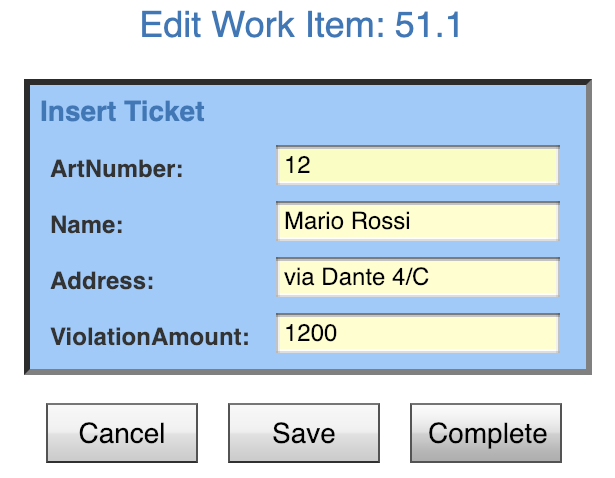
\includegraphics[scale=0.8]{ATCS/figures/insert.png}
        \caption{Front-end relativo al task \texttt{Insert Ticket}}
        \label{fig:insert}
    \end{figure}
    
    \noindent Una volta inserite queste informazioni, un utente della rete con il ruolo di "Prepare And Send" ha a disposizione 10 giorni per spedire la multa, altrimenti questa verrà considerata scaduta ed il flusso terminerà.
    
    \begin{figure}[h]
        \centering
        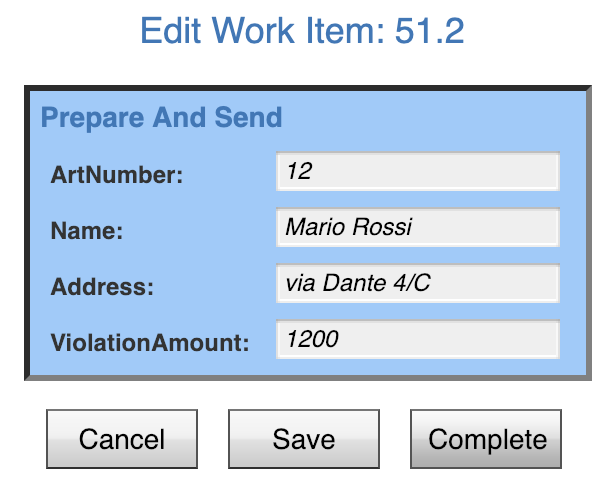
\includegraphics[scale=0.8]{ATCS/figures/prepare.png}
        \caption{Front-end relativo al task \texttt{Prepare And Send}}
        \label{fig:prepare}
    \end{figure}
    
    Nel caso in cui un operatore prepari ed invii la multa tramite il task \texttt{Prepare And Send}, permetterà la generazione di due token diversi attraverso uno split di tipo AND:
    \begin{itemize}
        \item Un token entra in una Deferred Choice (\texttt{Ticket Sent}). Questo implica che il task \texttt{Process Payment} verrà eseguito da un operatore di tipo "Processor" solo se si verificherà una determinata condizione. La condizione per la sua attivazione è la ricezione da parte del sistema di un pagamento (parziale o completo). L'operatore "Processor" inserirà la variabile \textit{AmountPaid} nella rete, questo provocherà l'esecuzione del task automatico \texttt{Add Amount}.
        
        \begin{figure}[h]
            \centering
            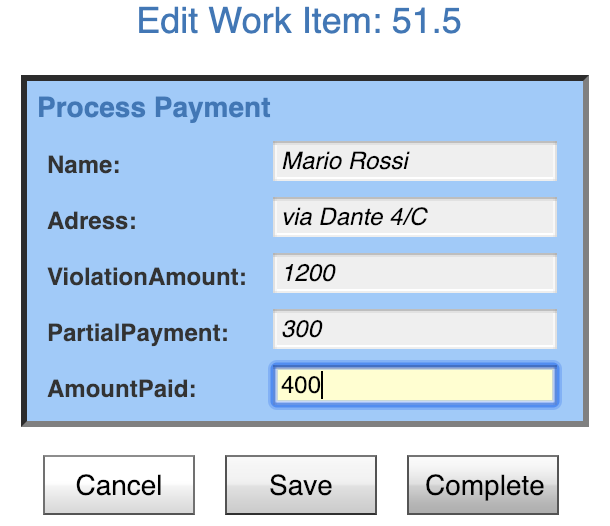
\includegraphics[scale=0.8]{ATCS/figures/payment.png}
            \caption{Front-end relativo al task \texttt{Process Payment}}
            \label{fig:pay}
        \end{figure}
        
        \noindent \texttt{Add Amount} (contrassegnato con l'icona di un ingranaggio) contiene un codelet di tipo XQueryEvaluator che, nella parte relativa alla \textbf{query}, non farà altro che sommare il valore contenuto all'interno della variabile \textit{AmountPaid} a quello della variabile \textit{SumPaid}. Il \textbf{result} della query sarà salvato all'interno della stessa variabile \textit{SumPaid} attraverso il "binding".\\
        Infine, \texttt{Add Amount} presenta uno split di tipo XOR la cui prima condizione permette di terminare il flusso nel caso in cui la somma contenuta all'interno di \textit{SumPaid} sia maggiore od uguale a quella totale che il trasgressore deve versare, contenuta in \textit{ViolationAmount}. Altrimenti, la condizione di default obbliga a tornare alla Deferred Choice \texttt{Ticket Sent};
        \item L'altro token provoca l'esecuzione di \texttt{Add Ticket For Credit Collection}, dopo aver aspettato 180 giorni. Questo limite temporale indica al trasgressore la scadenza per pagare la multa in toto. Dopo l'esecuzione del task il flusso termina e la multa è preparata per il "Recupero Crediti".
    \end{itemize}
    
    \subsection{Timers} Nella rete sono presenti \textbf{due timer} (nei task con l'icona della sveglia):
    \begin{enumerate}
        \item Il primo è relativo al task automatico \texttt{Archive The Ticket As Expired} e provoca la sua esecuzione dopo 10 giorni da quella di \texttt{Insert Ticket}, nel caso in cui non venga eseguito il task \texttt{Prepare And Send} prima dello scadere del tempo (regolamentato dalla Deferred Choice \texttt{Ticket Inserted});
        \item Il secondo è relativo al task automatico \texttt{Add Ticket For Credit Collection} e la sua esecuzione avviene dopo 180 giorni da quella di \texttt{Prepare And Send}.
    \end{enumerate}
    Entrambi i timer iniziano nel momento in cui viene offerta l'esecuzione del relativo task ("On offer") e scadono al termine della rispettiva durata ("After duration").
    \paragraph*{Osservazioni:} Durante l'esecuzione dei test abbiamo notato che il flusso non gestisce bene il caso particolare in cui la ricezione (parziale o totale) della somma da versare da parte del trasgressore sia ricevuta al \ang{180} giorno. È possibile che un operatore non riesca ad inserire in tempo i dati relativi all'importo e che la multa sia preparata per il "Recupero Crediti" nonostante sia stata saldata entro il tempo limite.\\
    Perciò, secondo noi, sarebbe ragionevole incrementare la durata del timer di un giorno lavorativo, che ci sembra un limite massimo corretto per permettere agli operatori "Processor" di eseguire il task \texttt{Process Payment}.
    
    \subsection{Cancellation Regions} Nella rete sono presenti due Cancellation Regions (nei task di colore blu).
    Il task \texttt{Prepare And Send} presenta uno split di tipo AND, ma nella rete non sono presenti degli AND join. È stato quindi necessario introdurre due Cancellation Regions per poter consumare il token rimasto rispettivamente nel flusso proveniente dall'AND split che non termina.
    \begin{enumerate}
        \item Nel caso in cui venga eseguito il task \texttt{Add Ticket For Credit Collection} il flusso termina cancellando anche il token presente nella sua Cancellation Region, formata da:
        \begin{itemize}
            \item \texttt{Ticket Sent};
            \item \texttt{Process Payment};
            \item \texttt{Add Amount}.
        \end{itemize}
        \item Nel caso, invece, in cui venga eseguito il task \texttt{dummy} (appositamente creato) il flusso termina cancellando anche il token presente nella sua Cancellation Region, formata da:
        \begin{itemize}
            \item \texttt{Add Ticket For Credit Collection}.
        \end{itemize}
    \end{enumerate}
    
\end{document}